\subsubsubsection{Kiến trúc pipeline 6 giai đoạn}

Để dung hòa giữa ràng buộc mềm (trải nghiệm người dùng) và ràng buộc cứng (logic toán học, vật lý), hệ thống TravelEZ không sử dụng phương pháp câu lệnh đơn. Thay vào đó, hệ thống áp dụng một pipeline gồm 6 giai đoạn nối tiếp được minh họa chi tiết trong Hình \ref{fig:pipeline_seq_diagram}.

Kiến trúc này tuân thủ nguyên lý trách nhiệm duy nhất, phân tách quá trình xử lý thành 6 bước tuần tự. Đầu ra của mỗi giai đoạn là đầu vào của giai đoạn tiếp theo, giúp kiểm soát luồng dữ liệu và giảm thiểu sai số.

\begin{figure}[htbp]
    \centering
    % Nhớ điều chỉnh lại đường dẫn file ảnh cho khớp với thư mục của bạn
    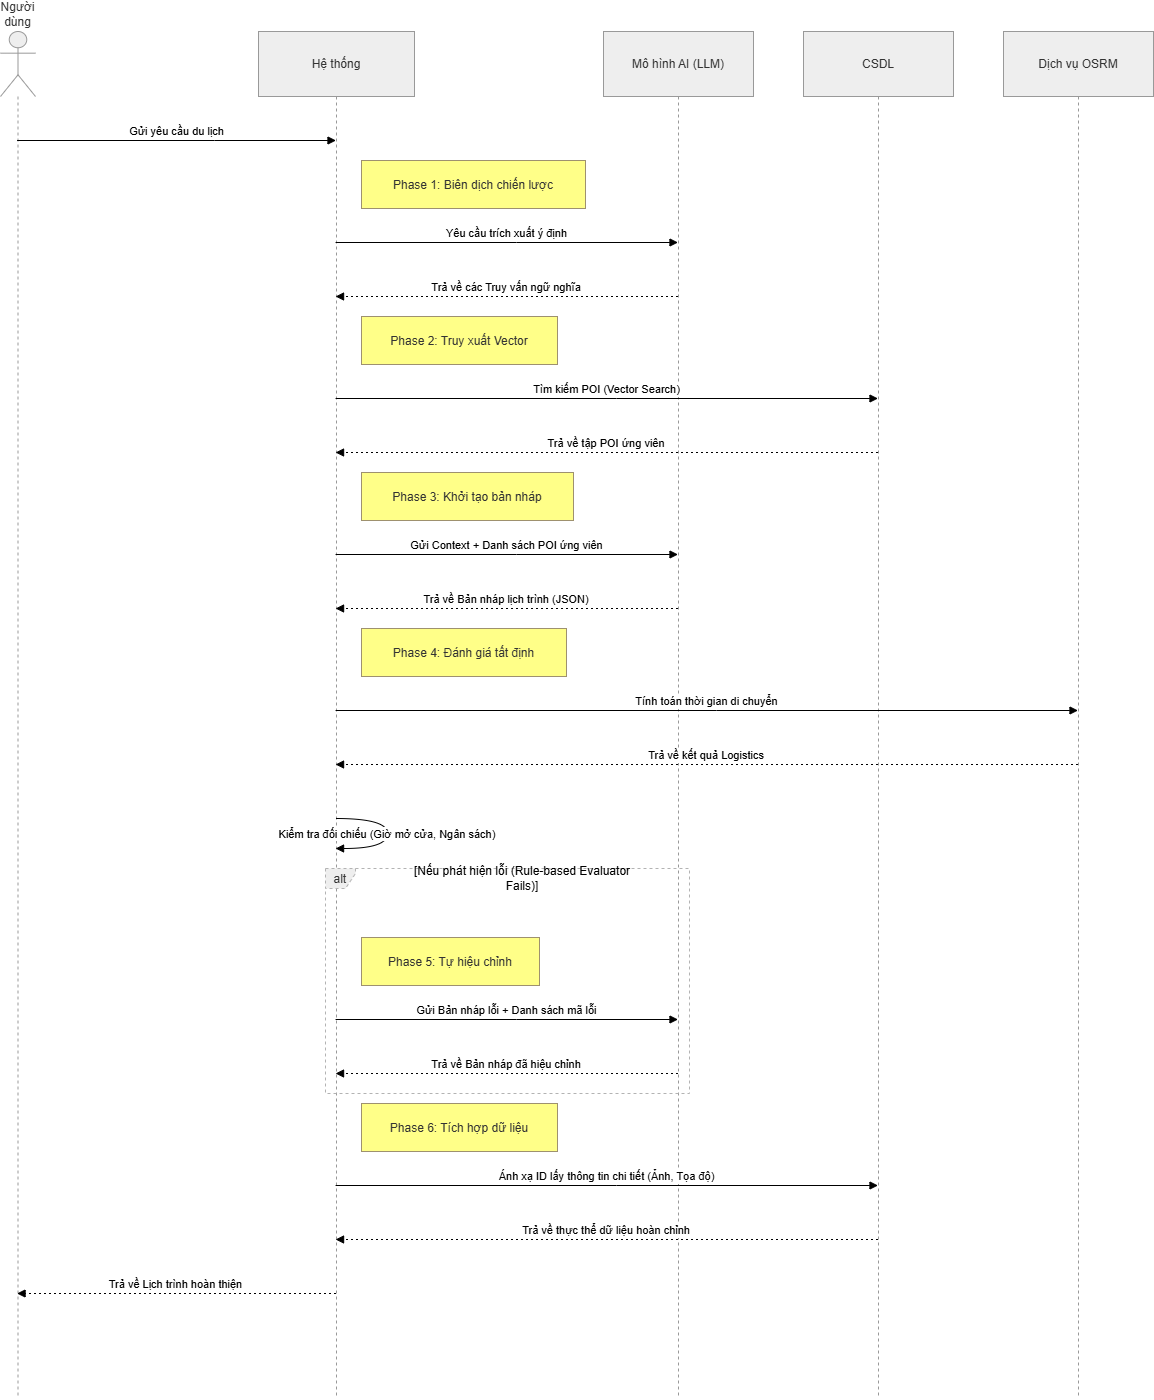
\includegraphics[width=0.9\textwidth]{Images/7. System Design/pipeline Itinerary.png}
    \caption{Biểu đồ tuần tự minh họa kiến trúc Pipeline 6 giai đoạn sinh lộ trình}
    \label{fig:pipeline_seq_diagram}
\end{figure}

\textbf{Giai đoạn 1: Biên dịch chiến lược}\\
\textbf{Mục tiêu:} Chuyển đổi yêu cầu ngôn ngữ tự nhiên không cấu trúc của người dùng thành các truy vấn có chủ đích.\\
\textbf{Chi tiết thực thi:} Hệ thống tiếp nhận cấu hình chuyến đi và các ghi chú cá nhân. Thay vì tìm kiếm trực tiếp, một mô hình LLM tốc độ cao được sử dụng để phân tích ngữ cảnh (như đặc điểm nhóm khách, hạn chế về thể chất) và biên dịch thành một tập hợp các truy vấn ngữ nghĩa (semantic queries). Các truy vấn này được định dạng bắt buộc với tiền tố phân loại (ví dụ: \textit{"Category: Restaurant. romantic and quiet"}), nhằm thiết lập cơ sở cho đối sánh vector.

\textbf{Giai đoạn 2: Truy xuất vector}\\
\textbf{Mục tiêu:} Cung cấp bộ nhớ ngữ cảnh chứa các điểm đến phù hợp nhất với ý định của người dùng.\\
\textbf{Chi tiết thực thi:} Triển khai phương pháp tìm kiếm lai. Các truy vấn từ giai đoạn 1 được chuyển đổi thành vector thông qua mô hình embedding. Trong cơ sở dữ liệu PostgreSQL với phần mở rộng \texttt{pgvector}, hệ thống kết hợp bộ lọc phân loại cứng (category) và toán tử khoảng cách cosine (\texttt{<=>}) để tìm kiếm K láng giềng gần nhất. Kết quả là một tập ứng viên (candidate pool) có độ tương đồng cao nhất về cảm xúc và trải nghiệm.

\textbf{Giai đoạn 3: Khởi tạo bản nháp}\\
\textbf{Mục tiêu:} Xử lý các ràng buộc mềm và phân bổ lịch trình sơ bộ theo cơ chế RAG.\\
\textbf{Chi tiết thực thi:} LLM đóng vai trò là bộ lập kế hoạch (planner), tiếp nhận cửa sổ ngữ cảnh (context window) bao gồm thông tin người dùng và tập dữ liệu POI ứng viên đã được xác thực. Thông qua kỹ thuật tinh chỉnh câu lệnh (prompt engineering), mô hình bị ràng buộc bởi các quy tắc trải nghiệm để sinh ra bản nháp lộ trình dưới định dạng JSON.

\textbf{Giai đoạn 4: Đánh giá tất định}\\
\textbf{Mục tiêu:} Đóng vai trò kiểm duyệt, bảo vệ các ràng buộc cứng mà AI có khả năng vi phạm.\\
\textbf{Chi tiết thực thi:} Bản nháp JSON được truyền qua một hệ thống thuật toán kiểm tra chéo, bao gồm:
\begin{itemize}
    \item \textit{Kiểm định không gian (Logistics):} Tích hợp công cụ Open Source Routing Machine (OSRM) để tính toán thời gian di chuyển vật lý giữa các tọa độ, đảm bảo các khoảng đệm thời gian là khả thi.
    \item \textit{Kiểm định thời gian (Operating hours):} Đối chiếu thời gian dự kiến diễn ra hoạt động với dữ liệu giờ mở/đóng cửa thực tế của POI trong cơ sở dữ liệu.
    \item \textit{Kiểm định tài chính (Budget):} Tính toán tổng chi phí dự kiến để đảm bảo nằm trong giới hạn ngân sách.
\end{itemize}
Kết quả là một báo cáo kiểm duyệt chứa danh sách các mã lỗi định lượng.

\textbf{Giai đoạn 5: Tự hiệu chỉnh}\\
\textbf{Mục tiêu:} Kích hoạt vòng lặp phản hồi để sửa các lỗi logic vật lý.\\
\textbf{Chi tiết thực thi:} Chỉ kích hoạt nếu báo cáo kiểm duyệt ở Giai đoạn 4 có lỗi. Mô-đun hiệu chỉnh nhận lại bản nháp ban đầu cùng danh sách mã lỗi, phân tích và thực hiện tái cấu trúc cục bộ (dịch chuyển thời gian, loại bỏ POI xung đột) để giải quyết triệt để ràng buộc cứng mà không phá vỡ ràng buộc mềm. Đầu ra là bản JSON đã được chuẩn hóa.

\textbf{Giai đoạn 6: Tích hợp dữ liệu}\\
\textbf{Mục tiêu:} Hoàn thiện đối tượng dữ liệu trước khi chuyển giao cho tầng giao diện.\\
\textbf{Chi tiết thực thi:} Giai đoạn cuối cùng thực hiện thao tác ánh xạ ngược các mã ID từ JSON vào cơ sở dữ liệu để truy xuất và đè/bổ sung các thông tin "chuẩn" như: hình ảnh đại diện, địa chỉ chi tiết, tọa độ bản đồ. Lộ trình lúc này trở thành một thực thể dữ liệu hoàn chỉnh, hoàn toàn loại bỏ nguy cơ "ảo giác dữ liệu" của AI.